% ---- Präambel mit Angaben zum Dokument
\documentclass[
	fontsize=12pt,           % Leitlinien sprechen von Schriftgröße 12.
	paper=A4,
	twoside=false,
]{scrreprt}                  % Verwendung von KOMA-Report
\usepackage[utf8]{inputenc}  % UTF8 Encoding einschalten
\usepackage[ngerman]{babel}  % Neue deutsche Rechtschreibung
\usepackage[T1]{fontenc}     % Ausgabe von westeuropäischen Zeichen (auch Umlaute)
\usepackage{graphicx}        % Einbinden von Grafiken erlauben
\usepackage{wrapfig}         % Grafiken fließend im Text
\usepackage{setspace}        % Zeilenabstand \singlespacing, \onehalfspaceing, \doublespacing
\usepackage{placeins}
\usepackage[
	%showframe,                % Ränder anzeigen lassen
	left=2.7cm, right=2.5cm,
	top=2.5cm,  bottom=2.5cm,
	includeheadfoot
]{geometry}                      % Seitenlayout einstellen
\usepackage{scrlayer-scrpage}    % Gestaltung von Fuß- und Kopfzeilen
\usepackage{acronym}             % Abkürzungen, Abkürzungsverzeichnis
\usepackage{titletoc}            % Anpassungen am Inhaltsverzeichnis
\contentsmargin{0.725cm}         % Abstand im Inhaltsverzeichnis zw. Punkt und Seitenzahl
\usepackage[                     % Klickbare Links (enth. auch "nameref", "url" Package)
  hidelinks,                     % Blende die "URL Boxen" aus.
  breaklinks=true                % Breche zu lange URLs am Zeilenende um
]{hyperref}
\urlstyle{same}                  % Aktuelle Schrift auch für URLs
% Anpassung von autoref für Gleichungen (ergänzt runde Klammern) und Algorithm.
% Anstatt "Listing" kann auch z.B. "Code-Ausschnitt" verwendet werden. Dies sollte
% jedoch synchron gehalten werden mit \lstlistingname (siehe weiter unten).
\addto\extrasngerman{%
	\def\equationautorefname~#1\null{Gleichung~(#1)\null}
	\def\lstnumberautorefname{Zeile}
	\def\lstlistingautorefname{Listing}
	\def\algorithmautorefname{Algorithmus}
	% Damit einheitlich "Abschnitt 1.2[.3]" verwendet wird und nicht "Unterabschnitt 1.2.3"
	% \def\subsectionautorefname{Abschnitt}
}

% ---- Abstand verkleinern von der Überschrift 
\renewcommand*{\chapterheadstartvskip}{\vspace*{.5\baselineskip}}

% Hierdurch werden Schusterjungen und Hurenkinder vermieden, d.h. einzelne Wörter
% auf der nächsten Seite oder in einer einzigen Zeile.
% LaTeX kann diese dennoch erzeugen, falls das Layout ansonsten nicht umsetzbar ist.
% Diese Werte sind aber gute Startwerte.
\widowpenalty10000
\clubpenalty10000

% ---- Für das Quellenverzeichnis
\usepackage[
	backend = biber,                % Verweis auf biber
	language = auto,
	style = numeric,                % Nummerierung der Quellen mit Zahlen
	sorting = none,                 % none = Sortierung nach der Erscheinung im Dokument
	sortcites = true,               % Sortiert die Quellen innerhalb eines cite-Befehls
	block = space,                  % Extra Leerzeichen zwischen Blocks
	hyperref = true,                % Links sind klickbar auch in der Quelle
	%backref = true,                % Referenz, auf den Text an die zitierte Stelle
	bibencoding = auto,
	giveninits = true,              % Vornamen werden abgekürzt
	doi=false,                      % DOI nicht anzeigen
	isbn=false,                     % ISBN nicht anzeigen
    alldates=short                  % Datum immer als DD.MM.YYYY anzeigen
]{biblatex}
%\addbibresource{Inhalt/literatur.bib}
\setcounter{biburlnumpenalty}{3000}     % Umbruchgrenze für Zahlen
\setcounter{biburlucpenalty}{6000}      % Umbruchgrenze für Großbuchstaben
\setcounter{biburllcpenalty}{9000}      % Umbruchgrenze für Kleinbuchstaben
\DeclareNameAlias{default}{last-first}  % Nachname vor dem Vornamen
\AtBeginBibliography{\renewcommand{\multinamedelim}{\addslash\space
}\renewcommand{\finalnamedelim}{\multinamedelim}}  % Schrägstrich zwischen den Autorennamen
\DefineBibliographyStrings{german}{
  urlseen = {Einsichtnahme:},                      % Ändern des Titels von "besucht am"
}
\usepackage[babel,german=quotes]{csquotes}         % Deutsche Anführungszeichen + Zitate


% ---- Für Mathevorlage
\usepackage{amsmath}    % Erweiterung vom Mathe-Satz
\usepackage{amssymb}    % Lädt amsfonts und weitere Symbole
\usepackage{MnSymbol}   % Für Symbole, die in amssymb nicht enthalten sind.


% ---- Für Quellcodevorlage
\usepackage{scrhack}                    % Hack zur Verw. von listings in KOMA-Script
\usepackage{listings}                   % Darstellung von Quellcode
\usepackage{color}                     % Einfache Verwendung von Farben

\usepackage{algorithm}                  % Für Algorithmen-Umgebung (ähnlich wie lstlistings Umgebung)
\usepackage{algpseudocode}              % Für Pseudocode. Füge "[noend]" hinzu, wenn du kein "endif",
                                        % etc. haben willst.

\makeatletter                           % Sorgt dafür, dass man @ in Namen verwenden kann.
                                        % Ansonsten gibt es in der nächsten Zeile einen Compilefehler.
\renewcommand{\ALG@name}{Algorithmus}   % Umbenennen von "Algorithm" im Header der Listings.
\makeatother                            % Zeichen wieder zurücksetzen
\renewcommand{\lstlistingname}{Listing} % Erlaubt das Umbenennen von "Listing" in anderen Titel.
\lstset{
  basicstyle=\ttfamily,
  columns=fullflexible,
  frame=single,
  breaklines=true,
  postbreak=\mbox{\textcolor{red}{$\hookrightarrow$}\space},
}

% ---- Tabellen
\usepackage{booktabs}  % Für schönere Tabellen. Enthält neue Befehle wie \midrule
\usepackage{multirow}  % Mehrzeilige Tabellenkein Punkt verwendet wird.

% ---- Für Definitionsboxen in der Einleitung
\usepackage{amsthm}                     % Liefert die Grundlagen für Theoreme
\usepackage[framemethod=tikz]{mdframed} % Boxen für die Umrandung

% ---- Für Todo Notes
\usepackage{todonotes}
\lstdefinelanguage{Rust}{%
  sensitive%
, morecomment=[l]{//}%
, morecomment=[s]{/*}{*/}%
, moredelim=[s][{\itshape\color[rgb]{0,0,0.75}}]{\#[}{]}%
, morestring=[b]{"}%
, alsodigit={}%
, alsoother={}%
, alsoletter={!}%
%
%
% [1] reserve keywords
% [2] traits
% [3] primitive types
% [4] type and value constructors
% [5] identifier
%
, morekeywords={break, continue, else, for, if, in, loop, match, return, while}  % control flow keywords
, morekeywords={as, const, let, move, mut, ref, static}  % in the context of variables
, morekeywords={dyn, enum, fn, impl, Self, self, struct, trait, type, union, use, where}  % in the context of declarations
, morekeywords={crate, extern, mod, pub, super}  % in the context of modularisation
, morekeywords={unsafe}  % markers
, morekeywords={abstract, alignof, become, box, do, final, macro, offsetof, override, priv, proc, pure, sizeof, typeof, unsized, virtual, yield}  % reserved identifiers
%
% grep 'pub trait [A-Za-z][A-Za-z0-9]*' -r . | sed 's/^.*pub trait \([A-Za-z][A-Za-z0-9]*\).*/\1/g' | sort -u | tr '\n' ',' | sed 's/^\(.*\),$/{\1}\n/g' | sed 's/,/, /g'
, morekeywords=[2]{Add, AddAssign, Any, AsciiExt, AsInner, AsInnerMut, AsMut, AsRawFd, AsRawHandle, AsRawSocket, AsRef, Binary, BitAnd, BitAndAssign, Bitor, BitOr, BitOrAssign, BitXor, BitXorAssign, Borrow, BorrowMut, Boxed, BoxPlace, BufRead, BuildHasher, CastInto, CharExt, Clone, CoerceUnsized, CommandExt, Copy, Debug, DecodableFloat, Default, Deref, DerefMut, DirBuilderExt, DirEntryExt, Display, Div, DivAssign, DoubleEndedIterator, DoubleEndedSearcher, Drop, EnvKey, Eq, Error, ExactSizeIterator, ExitStatusExt, Extend, FileExt, FileTypeExt, Float, Fn, FnBox, FnMut, FnOnce, Freeze, From, FromInner, FromIterator, FromRawFd, FromRawHandle, FromRawSocket, FromStr, FullOps, FusedIterator, Generator, Hash, Hasher, Index, IndexMut, InPlace, Int, Into, IntoCow, IntoInner, IntoIterator, IntoRawFd, IntoRawHandle, IntoRawSocket, IsMinusOne, IsZero, Iterator, JoinHandleExt, LargeInt, LowerExp, LowerHex, MetadataExt, Mul, MulAssign, Neg, Not, Octal, OpenOptionsExt, Ord, OsStrExt, OsStringExt, Packet, PartialEq, PartialOrd, Pattern, PermissionsExt, Place, Placer, Pointer, Product, Put, RangeArgument, RawFloat, Read, Rem, RemAssign, Seek, Shl, ShlAssign, Shr, ShrAssign, Sized, SliceConcatExt, SliceExt, SliceIndex, Stats, Step, StrExt, Sub, SubAssign, Sum, Sync, TDynBenchFn, Terminal, Termination, ToOwned, ToSocketAddrs, ToString, Try, TryFrom, TryInto, UnicodeStr, Unsize, UpperExp, UpperHex, WideInt, Write}
, morekeywords=[2]{Send}  % additional traits
%
, morekeywords=[3]{bool, char, f32, f64, i8, i16, i32, i64, isize, str, u8, u16, u32, u64, unit, usize, i128, u128}  % primitive types
%
, morekeywords=[4]{Err, false, None, Ok, Some, true}  % prelude value constructors
% grep 'pub \(type\|struct\|enum\) [A-Za-z][A-Za-z0-9]*' -r . | sed 's/^.*pub \(type\|struct\|enum\) \([A-Za-z][A-Za-z0-9]*\).*/\2/g' | sort -u | tr '\n' ',' | sed 's/^\(.*\),$/{\1}\n/g' | sed 's/,/, /g'    
, morekeywords=[3]{AccessError, Adddf3, AddI128, AddoI128, AddoU128, ADDRESS, ADDRESS64, addrinfo, ADDRINFOA, AddrParseError, Addsf3, AddU128, advice, aiocb, Alignment, AllocErr, AnonPipe, Answer, Arc, Args, ArgsInnerDebug, ArgsOs, Argument, Arguments, ArgumentV1, Ashldi3, Ashlti3, Ashrdi3, Ashrti3, AssertParamIsClone, AssertParamIsCopy, AssertParamIsEq, AssertUnwindSafe, AtomicBool, AtomicPtr, Attr, auxtype, auxv, BackPlace, BacktraceContext, Barrier, BarrierWaitResult, Bencher, BenchMode, BenchSamples, BinaryHeap, BinaryHeapPlace, blkcnt, blkcnt64, blksize, BOOL, boolean, BOOLEAN, BoolTrie, BorrowError, BorrowMutError, Bound, Box, bpf, BTreeMap, BTreeSet, Bucket, BucketState, Buf, BufReader, BufWriter, Builder, BuildHasherDefault, BY, BYTE, Bytes, CannotReallocInPlace, cc, Cell, Chain, CHAR, CharIndices, CharPredicateSearcher, Chars, CharSearcher, CharsError, CharSliceSearcher, CharTryFromError, Child, ChildPipes, ChildStderr, ChildStdin, ChildStdio, ChildStdout, Chunks, ChunksMut, ciovec, clock, clockid, Cloned, cmsgcred, cmsghdr, CodePoint, Color, ColorConfig, Command, CommandEnv, Component, Components, CONDITION, condvar, Condvar, CONSOLE, CONTEXT, Count, Cow, cpu, CRITICAL, CStr, CString, CStringArray, Cursor, Cycle, CycleIter, daddr, DebugList, DebugMap, DebugSet, DebugStruct, DebugTuple, Decimal, Decoded, DecodeUtf16, DecodeUtf16Error, DecodeUtf8, DefaultEnvKey, DefaultHasher, dev, device, Difference, Digit32, DIR, DirBuilder, dircookie, dirent, dirent64, DirEntry, Discriminant, DISPATCHER, Display, Divdf3, Divdi3, Divmoddi4, Divmodsi4, Divsf3, Divsi3, Divti3, dl, Dl, Dlmalloc, Dns, DnsAnswer, DnsQuery, dqblk, Drain, DrainFilter, Dtor, Duration, DwarfReader, DWORD, DWORDLONG, DynamicLibrary, Edge, EHAction, EHContext, Elf32, Elf64, Empty, EmptyBucket, EncodeUtf16, EncodeWide, Entry, EntryPlace, Enumerate, Env, epoll, errno, Error, ErrorKind, EscapeDebug, EscapeDefault, EscapeUnicode, event, Event, eventrwflags, eventtype, ExactChunks, ExactChunksMut, EXCEPTION, Excess, ExchangeHeapSingleton, exit, exitcode, ExitStatus, Failure, fd, fdflags, fdsflags, fdstat, ff, fflags, File, FILE, FileAttr, filedelta, FileDesc, FilePermissions, filesize, filestat, FILETIME, filetype, FileType, Filter, FilterMap, Fixdfdi, Fixdfsi, Fixdfti, Fixsfdi, Fixsfsi, Fixsfti, Fixunsdfdi, Fixunsdfsi, Fixunsdfti, Fixunssfdi, Fixunssfsi, Fixunssfti, Flag, FlatMap, Floatdidf, FLOATING, Floatsidf, Floatsisf, Floattidf, Floattisf, Floatundidf, Floatunsidf, Floatunsisf, Floatuntidf, Floatuntisf, flock, ForceResult, FormatSpec, Formatted, Formatter, Fp, FpCategory, fpos, fpos64, fpreg, fpregset, FPUControlWord, Frame, FromBytesWithNulError, FromUtf16Error, FromUtf8Error, FrontPlace, fsblkcnt, fsfilcnt, fsflags, fsid, fstore, fsword, FullBucket, FullBucketMut, FullDecoded, Fuse, GapThenFull, GeneratorState, gid, glob, glob64, GlobalDlmalloc, greg, group, GROUP, Guard, GUID, Handle, HANDLE, Handler, HashMap, HashSet, Heap, HINSTANCE, HMODULE, hostent, HRESULT, id, idtype, if, ifaddrs, IMAGEHLP, Immut, in, in6, Incoming, Infallible, Initializer, ino, ino64, inode, input, InsertResult, Inspect, Instant, int16, int32, int64, int8, integer, IntermediateBox, Internal, Intersection, intmax, IntoInnerError, IntoIter, IntoStringError, intptr, InvalidSequence, iovec, ip, IpAddr, ipc, Ipv4Addr, ipv6, Ipv6Addr, Ipv6MulticastScope, Iter, IterMut, itimerspec, itimerval, jail, JoinHandle, JoinPathsError, KDHELP64, kevent, kevent64, key, Key, Keys, KV, l4, LARGE, lastlog, launchpad, Layout, Lazy, lconv, Leaf, LeafOrInternal, Lines, LinesAny, LineWriter, linger, linkcount, LinkedList, load, locale, LocalKey, LocalKeyState, Location, lock, LockResult, loff, LONG, lookup, lookupflags, LookupHost, LPBOOL, LPBY, LPBYTE, LPCSTR, LPCVOID, LPCWSTR, LPDWORD, LPFILETIME, LPHANDLE, LPOVERLAPPED, LPPROCESS, LPPROGRESS, LPSECURITY, LPSTARTUPINFO, LPSTR, LPVOID, LPWCH, LPWIN32, LPWSADATA, LPWSAPROTOCOL, LPWSTR, Lshrdi3, Lshrti3, lwpid, M128A, mach, major, Map, mcontext, Metadata, Metric, MetricMap, mflags, minor, mmsghdr, Moddi3, mode, Modsi3, Modti3, MonitorMsg, MOUNT, mprot, mq, mqd, msflags, msghdr, msginfo, msglen, msgqnum, msqid, Muldf3, Mulodi4, Mulosi4, Muloti4, Mulsf3, Multi3, Mut, Mutex, MutexGuard, MyCollection, n16, NamePadding, NativeLibBoilerplate, nfds, nl, nlink, NodeRef, NoneError, NonNull, NonZero, nthreads, NulError, OccupiedEntry, off, off64, oflags, Once, OnceState, OpenOptions, Option, Options, OptRes, Ordering, OsStr, OsString, Output, OVERLAPPED, Owned, Packet, PanicInfo, Param, ParseBoolError, ParseCharError, ParseError, ParseFloatError, ParseIntError, ParseResult, Part, passwd, Path, PathBuf, PCONDITION, PCONSOLE, Peekable, PeekMut, Permissions, PhantomData, pid, Pipes, PlaceBack, PlaceFront, PLARGE, PoisonError, pollfd, PopResult, port, Position, Powidf2, Powisf2, Prefix, PrefixComponent, PrintFormat, proc, Process, PROCESS, processentry, protoent, PSRWLOCK, pthread, ptr, ptrdiff, PVECTORED, Queue, radvisory, RandomState, Range, RangeFrom, RangeFull, RangeInclusive, RangeMut, RangeTo, RangeToInclusive, RawBucket, RawFd, RawHandle, RawPthread, RawSocket, RawTable, RawVec, Rc, ReadDir, Receiver, recv, RecvError, RecvTimeoutError, ReentrantMutex, ReentrantMutexGuard, Ref, RefCell, RefMut, REPARSE, Repeat, Result, Rev, Reverse, riflags, rights, rlim, rlim64, rlimit, rlimit64, roflags, Root, RSplit, RSplitMut, RSplitN, RSplitNMut, RUNTIME, rusage, RwLock, RWLock, RwLockReadGuard, RwLockWriteGuard, sa, SafeHash, Scan, sched, scope, sdflags, SearchResult, SearchStep, SECURITY, SeekFrom, segment, Select, SelectionResult, sem, sembuf, send, Sender, SendError, servent, sf, Shared, shmatt, shmid, ShortReader, ShouldPanic, Shutdown, siflags, sigaction, SigAction, sigevent, sighandler, siginfo, Sign, signal, signalfd, SignalToken, sigset, sigval, Sink, SipHasher, SipHasher13, SipHasher24, size, SIZE, Skip, SkipWhile, Slice, SmallBoolTrie, sockaddr, SOCKADDR, sockcred, Socket, SOCKET, SocketAddr, SocketAddrV4, SocketAddrV6, socklen, speed, Splice, Split, SplitMut, SplitN, SplitNMut, SplitPaths, SplitWhitespace, spwd, SRWLOCK, ssize, stack, STACKFRAME64, StartResult, STARTUPINFO, stat, Stat, stat64, statfs, statfs64, StaticKey, statvfs, StatVfs, statvfs64, Stderr, StderrLock, StderrTerminal, Stdin, StdinLock, Stdio, StdioPipes, Stdout, StdoutLock, StdoutTerminal, StepBy, String, StripPrefixError, StrSearcher, subclockflags, Subdf3, SubI128, SuboI128, SuboU128, subrwflags, subscription, Subsf3, SubU128, Summary, suseconds, SYMBOL, SYMBOLIC, SymmetricDifference, SyncSender, sysinfo, System, SystemTime, SystemTimeError, Take, TakeWhile, tcb, tcflag, TcpListener, TcpStream, TempDir, TermInfo, TerminfoTerminal, termios, termios2, TestDesc, TestDescAndFn, TestEvent, TestFn, TestName, TestOpts, TestResult, Thread, threadattr, threadentry, ThreadId, tid, time, time64, timespec, TimeSpec, timestamp, timeval, timeval32, timezone, tm, tms, ToLowercase, ToUppercase, TraitObject, TryFromIntError, TryFromSliceError, TryIter, TryLockError, TryLockResult, TryRecvError, TrySendError, TypeId, U64x2, ucontext, ucred, Udivdi3, Udivmoddi4, Udivmodsi4, Udivmodti4, Udivsi3, Udivti3, UdpSocket, uid, UINT, uint16, uint32, uint64, uint8, uintmax, uintptr, ulflags, ULONG, ULONGLONG, Umoddi3, Umodsi3, Umodti3, UnicodeVersion, Union, Unique, UnixDatagram, UnixListener, UnixStream, Unpacked, UnsafeCell, UNWIND, UpgradeResult, useconds, user, userdata, USHORT, Utf16Encoder, Utf8Error, Utf8Lossy, Utf8LossyChunk, Utf8LossyChunksIter, utimbuf, utmp, utmpx, utsname, uuid, VacantEntry, Values, ValuesMut, VarError, Variables, Vars, VarsOs, Vec, VecDeque, vm, Void, WaitTimeoutResult, WaitToken, wchar, WCHAR, Weak, whence, WIN32, WinConsole, Windows, WindowsEnvKey, winsize, WORD, Wrapping, wrlen, WSADATA, WSAPROTOCOL, WSAPROTOCOLCHAIN, Wtf8, Wtf8Buf, Wtf8CodePoints, xsw, xucred, Zip, zx}
%
, morekeywords=[5]{assert!, assert_eq!, assert_ne!, cfg!, column!, compile_error!, concat!, concat_idents!, debug_assert!, debug_assert_eq!, debug_assert_ne!, env!, eprint!, eprintln!, file!, format!, format_args!, include!, include_bytes!, include_str!, line!, module_path!, option_env!, panic!, print!, println!, select!, stringify!, thread_local!, try!, unimplemented!, unreachable!, vec!, write!, writeln!}  % prelude macros
}%

\lstdefinestyle{colouredRust}%
{ basicstyle=\ttfamily%
, identifierstyle=%
, commentstyle=\color[gray]{0.4}%
, stringstyle=\color[rgb]{0, 0, 0.5}%
, keywordstyle=\bfseries% reserved keywords
, keywordstyle=[2]\color[rgb]{0.75, 0, 0}% traits
, keywordstyle=[3]\color[rgb]{0, 0.5, 0}% primitive types
, keywordstyle=[4]\color[rgb]{0, 0.5, 0}% type and value constructors
, keywordstyle=[5]\color[rgb]{0, 0, 0.75}% macros
, columns=spaceflexible%
, keepspaces=true%
, showspaces=false%
, showtabs=false%
, showstringspaces=true%
}%

\lstdefinestyle{boxed}{
  style=colouredRust%
, numbers=left%
, firstnumber=auto%
, numberblanklines=true%
, frame=trbL%
, numberstyle=\tiny%
, frame=leftline%
, numbersep=7pt%
, framesep=5pt%
, framerule=10pt%
, xleftmargin=15pt%
, backgroundcolor=\color[gray]{0.97}%
, rulecolor=\color[gray]{0.90}%
}

\usepackage{ifthen}

% ---- Persönlichen Daten:
\newcommand{\titel}{Aufgabe zu HashSets}
\newcommand{\titelheader}{Aufgabe zu HashSets}
\newcommand{\arbeit}{Aufgabe zu HashSets}
\newcommand{\autor}{Erik Imgrund}
\newcommand{\autorReverse}{Imgrund, Erik}
\newcommand{\kurs}{TINF19B1}

% ---- Metainformation für das PDF Dokument
\hypersetup{
	pdftitle    = {\titel},
	pdfsubject  = {\arbeit},
	pdfauthor   = {\autor},
	%pdfkeywords = {Keywords angeben},
	pdfcreator  = {LaTeX},
	%pdfproducer = {in der Regel pdfTeX}
}

% ---- Definition der Kopf- und Fußzeilen
\clearscrheadfoot                               % Löschen von LaTeX Standard
\automark[section]{chapter}                     % Füllen von section und chapter
\renewcommand*{\chaptermarkformat}{}            % Entfernt die Kapitelnummer
\renewcommand*{\sectionmarkformat}{}            % Entfernt die Sectionnummer
% Angaben [für "plain"]{für "scrheadings"}
\ihead[]{\titelheader}                          % Kopfzeile links
\chead[]{}                                      % Kopfzeile mitte
\ohead[]{\rightmark}                            % Kopfzeile rechts
\ifoot[]{}                                      % Fußzeile links
\cfoot*{\sffamily\pagemark}                     % Fußzeile mitte
\ofoot[]{}                                      % Fußzeile rechts
\KOMAoptions{
   headsepline = 0.2pt,                         % Liniendicke Kopfzeile
   footsepline = false                          % Liniendicke Fußzeile
}

% ---- Hilfreiches
\newcommand{\zB}{z.\,B. }
\newcommand{\dash}{d.\,h. }

\newcommand{\code}[1]{\texttt{#1}} % Ist einfacher zu schreiben als ständig \texttt und erlaubt
                                   % Änderungen im Nachhinein, wenn man z.B. Inline-Code anders stylen möchte.


% ---- Beginn des Dokuments
\begin{document}
\setlength{\parindent}{0pt}              % Keine Paragraphen Einrückung.
                                         % Dafür haben wir den Abstand zwischen den Paragraphen.
\setcounter{secnumdepth}{2}              % Nummerierungstiefe fürs Inhaltsverzeichnis
\setcounter{tocdepth}{1}                 % Tiefe des Inhaltsverzeichnisses. Ggf. so anpassen,
                                         % dass das Verzeichnis auf eine Seite passt.
\sffamily                                % Serifenlose Schrift verwenden.

% ---- Vorspann
% ------ Titelseite
\singlespacing
\newcounter{savepage}
\pagenumbering{Roman}                    % Römische Seitenzahlen
\onehalfspacing

% ------ Inhaltsverzeichnis
\singlespacing
\title{Aufgabe zu HashSets}
\author{Erik Imgrund, TINF19B1}
\maketitle
% \tableofcontents

% ------ Verzeichnisse
% \renewcommand*{\chapterpagestyle}{plain}
% \pagestyle{plain}
% \renewcommand{\lstlistlistingname}{Quellcodeverzeichnis}
% \lstlistoflistings                      % Erzeugen des Listenverzeichnisses
\setcounter{savepage}{\value{page}}


% ---- Inhalt der Arbeit
\cleardoublepage
\pagenumbering{arabic}                  % Arabische Seitenzahlen für den Hauptteil
\setlength{\parskip}{0.5\baselineskip}  % Abstand zwischen Absätzen
\rmfamily
\renewcommand*{\chapterpagestyle}{scrheadings}
\pagestyle{scrheadings}
\onehalfspacing
\chapter{Grundlegendes}
\section{Verwendete Verfahren}
Zur Kollisionsauflösung wurden Direct Chaining, Separate Chaining, Linear Probing, Quadratic Probing, Triangular Probing und ein Coalesced Table implementiert. Als Hashfunktionen wurden einmal der simple ModHash und MulHash aus der Vorlesung implementiert, sowie ein gebräuchlicher XorShiftHash. Bei dem XorShiftHash wird die Zahl mit einer Konstante multipliziert, bitweise verschoben und dann über ein bitweises Exklusiv-Oder mit der nicht-verschobenen Variante kombiniert.
\section{Aufgabestellung}
In der Aufgabe wurde beschrieben, dass mit konstanter Anzahl an Buckets und unter verschiedenen Lastfaktoren die Anzahl an Kollisionen pro Zugriff und \enquote{was für sinnvoll gehalten wird} gemessen werden soll. Für sinnvoll wird gehalten, die Zugriffszeit zu messen, dementsprechend wurde dieses auch getan.

Für sinnvoll wurde ebenfalls gehalten, die Messungen unter anderen Bedingungen zu wiederholen. Da jeder Bucket eines OpenAddressingTables nur 8 Byte groß ist, einer eines CoalescedTables jedoch 24 Byte könnte bei gleichem Speicherverbauch ein 3 mal so großer OpenAddressingTable erstellt werden. Die Messung mit konstanter Anzahl an Buckets benachteiligt stark OpenAddressingTables, deswegen wurde eine zweite Messreihe mit angepassten Größen durchgeführt. Die Herleitung der verwendeten Anzahl an Buckets pro Verfahren ist im Folgenden zu finden.

\section{Anzahl an Buckets in Abhängigkeit der geforderten Speichergröße}
Die Speichergröße wird festgelegt auf die Größe eines OpenAddressingTables mit $2^{15}$ Buckets, das entspricht 262kB. Für den CoalescedTable sind Buckets 24B groß, also werden $\frac{262kB}{24B} = 10922$ Buckets verwendet.

Für DirectChainingTables ist ein Bucket ebenfalls 8 Byte groß, jedoch werden zusätzlich für jedes Element 16B alloziiert, daher wird vom vorhandanden Speicherlimit zuerst die Anzahl der Elemente multipliziert mit der Größe eines Elements abgezogen und danach die größtmögliche Anzahl an Buckets im Restspeicherplatz alloziiert.

Für SeparateChainingTables ist das Verfahren komplizierter, da bloß Speicherplatz für jedes Element, welches mit einem anderen kollidiert Extra-Platz alloziiert werden muss. Dafür wird dafür ausgegangen, dass grundlegend jedes eingefügte Element 16B Speicherplatz benötigt, jeder leer gebliebene Bucket am Ende des Einfügens jedoch auch 16B. Die Wahrscheinlichkeit, dass ein bestimmter Bucket nach dem Einfügen von $n$ Elementen noch leer ist ist direkt abhängig von der Anzahl der Buckets $m$ und ergibt sich als $p = \left(\frac{m-1}{m}\right)^n$. Der Erwartungswert leerer Buckets ist somit $E = m\left(\frac{m-1}{m}\right)^n$ und der verwendete Platz ist $N = 16B\left(n + m\left(\frac{m-1}{m}\right)^n\right)$. Diese Gleichung wird numerisch für ein möglichst großes $m$ gelöst, für welches $N \le 262kB$ gilt.
\chapter{Ergebnisse}
\section{Ergebnisse bei Messung nach Aufgabenbedingungen}
\begin{table}[h!]
\begin{tabular}{c|cccc}
    Name & 50\% & 90\% & 95\% & 100\% \\
    \hline
    Quadratic Mul & 0,42 & 1,73 & 2,35 & 8,8 \\
    Quadratic Mod & 0,44 & 1,72 & 2,32 & 10,38 \\
    Quadratic XOR & 0,43 & 1,71 & 2,36 & 9,54 \\
    \hline
    Linear Mul & 0,43 & 1,87 & 2,60 & 8,93 \\
    Linear Mod & 0,42 & 1,87 & 2,64 & 10,51 \\
    Linear XOR & 0,44 & 1,91 & 2,59 & 9,83 \\
    \hline
    Triangular Mul & 0,42 & 1,71 & 2,36 & 8,85 \\
    Triangular Mod & 0,43 & 1,74 & 2,37 & 8,12 \\
    Triangular XOR & 0,43 & 1,69 & 2,35 & 9,71 \\
    \hline
    Direct Mul & 0,25 & 0,44 & 0,47 & 0,50 \\
    Direct Mod & 0,26 & 0,45 & 0,48 & 0,50 \\
    Direct XOR & 0,25 & 0,45 & 0,48 & 0,51 \\
    \hline
    Separate Mul & 0,24 & 0,44 & 0,48 & 0,50 \\
    Separate Mod & 0,25 & 0,45 & 0,47 & 0,50 \\
    Separate XOR & 0,25 & 0,46 & 0,48 & 0,51 \\
    \hline
    Coalesced Mul & 1,17 & 1,66 & 1,74 & 1,80 \\
    Coalesced Mod & 1,16 & 1,66 & 1,72 & 1,79 \\
    Coalesced XOR & 1,17 & 1,65 & 1,72 & 1,79 \\
\end{tabular}
\centering
\caption{Durchschnittliche Kollisionen bei Zugriff mit Erfolg}
\end{table}
\begin{table}[h!]
\begin{tabular}{c|cccc}
    Name & 50\% & 90\% & 95\% & 100\% \\
    \hline
    Quadratic Mul & 1,14 & 9,50 & 19,51 & - \\
    Quadratic Mod & 1,14 & 9,60 & 19,73 & - \\
    Quadratic XOR & 1,13 & 9,62 & 19,73 & - \\
    \hline
    Linear Mul & 1,16 & 11,14 & 22,45 & - \\
    Linear Mod & 1,16 & 11,01 & 23,09 & - \\
    Linear XOR & 1,17 & 11,14 & 24,24 & - \\
    \hline
    Triangular Mul & 1,12 & 9,72 & 19,94 & - \\
    Triangular Mod & 1,13 & 9,69 & 19,68 & - \\
    Triangular XOR & 1,13 & 9,74 & 19,58 & - \\
    \hline
    Direct Mul & 0,50 & 0,90 & 0,95 & 0,99 \\
    Direct Mod & 0,50 & 0,91 & 0,94 & 1,00 \\
    Direct XOR & 0,50 & 0,90 & 0,95 & 0,99 \\
    \hline
    Separate Mul & 0,50 & 0,90 & 0,95 & 0,99 \\
    Separate Mod & 0,50 & 0,90 & 0,96 & 1,00 \\
    Separate XOR & 0,50 & 0,90 & 0,95 & 1,00 \\
    \hline
    Coalesced Mul & 2,19 & 2,84 & 2,97 & 3,09 \\
    Coalesced Mod & 2,18 & 2,84 & 2,94 & 3,10 \\
    Coalesced XOR & 2,18 & 2,80 & 2,93 & 3,06 \\
\end{tabular}
\centering
\caption{Durchschnittliche Kollisionen bei Zugriff mit Erfolg}
\end{table}
\begin{table}[h!]
\begin{tabular}{c|cccc}
    Name & 50\% & 90\% & 95\% & 100\% \\
    \hline
    Quadratic Mul & 15,69 & 22,84 & 26,38 & 36,12 \\
    Quadratic Mod & 7,95 & 12,98 & 17,40 & 26,56 \\
    Quadratic XOR & 11,11 & 19,13 & 13,36 & 26,82 \\
    \hline
    Linear Mul & 22,36 & 18,60 & 18,47 & 28,08 \\
    Linear Mod & 7,07 & 11,77 & 12,42 & 21,82 \\
    Linear XOR & 12,34 & 16,40 & 13,42 & 42,18 \\
    \hline
    Triangular Mul & 12,73 & 22,71 & 19,54 & 44,04 \\
    Triangular Mod & 6,40 & 11,02 & 11,95 & 20,09 \\
    Triangular XOR & 8,25 & 14,00 & 13,82 & 27,00 \\
    \hline
    Direct Mul & 29,27 & 18,00 & 18,34 & 18,84 \\
    Direct Mod & 11,03 & 30,81 & 15,37  & 15,18 \\
    Direct XOR & 15,89 & 16,96 & 17,24  & 19,36 \\
    \hline
    Separate Mul & 11,61 & 15,89 & 22,11 & 24,84 \\
    Separate Mod & 8,80 & 12,73 & 25,38 & 13,32 \\
    Separate XOR & 10,45 & 14,45 & 14,89 & 21,30 \\
    \hline
    Coalesced Mul & 13,39 & 22,21 & 18,46 & 18,33 \\
    Coalesced Mod & 10,66 & 15,11 & 16,11 & 15,69 \\
    Coalesced XOR & 12,40 & 23,61 & 16,96 & 18,37 \\
\end{tabular}
\centering
\caption{Durchschnittliche Kollisionen bei Zugriff mit Erfolg}
\end{table}
\begin{table}[h!]
\begin{tabular}{c|cccc}
    Name & 50\% & 90\% & 95\% & 100\% \\
    \hline
    Quadratic Mul & 26,70 & 54,74 & 63,56 & - \\
    Quadratic Mod & 29,43 & 34,32 & 47,58 & - \\
    Quadratic XOR & 23,65 & 33,29 & 42,50 & - \\
    \hline
    Linear Mul & 28,92 & 43,14 & 49,96 & - \\
    Linear Mod & 17,75 & 34,40 & 41,58 & - \\
    Linear XOR & 21,51 & 32,34 & 45,58 & - \\
    \hline
    Triangular Mul & 24,55 & 45,98 & 51,65 & - \\
    Triangular Mod & 16,08 & 29,74 & 42,57 & - \\
    Triangular XOR & 19,55 & 33,58 & 45,38 & - \\
    \hline
    Direct Mul & 31,02 & 30,57 & 31,61 & 31,03 \\
    Direct Mod & 19,57 & 38,78 & 26,45 & 26,70 \\
    Direct XOR & 23,20 & 44,13 & 29,42 & 30,70 \\
    \hline
    Separate Mul & 23,49 & 28,22 & 30,52 & 31,97 \\
    Separate Mod & 27,56 & 23,86 & 34,34 & 24,72 \\
    Separate XOR & 22,51 & 27,11 & 27,73 & 29,54 \\
    \hline
    Coalesced Mul & 18,64 & 33,36 & 31,12 & 32,21 \\
    Coalesced Mod & 15,82 & 25,53 & 32,82 & 29,31 \\
    Coalesced XOR & 17,42 & 34,61 & 30,27 & 32,26 \\
\end{tabular}
\centering
\caption{Durchschnittliche Kollisionen bei Zugriff mit Erfolg}
\end{table}
\FloatBarrier
\section{Ergebnisse bei Messung nach für sinnvoll gehaltenen Bedingungen}
\begin{figure}[h!]
    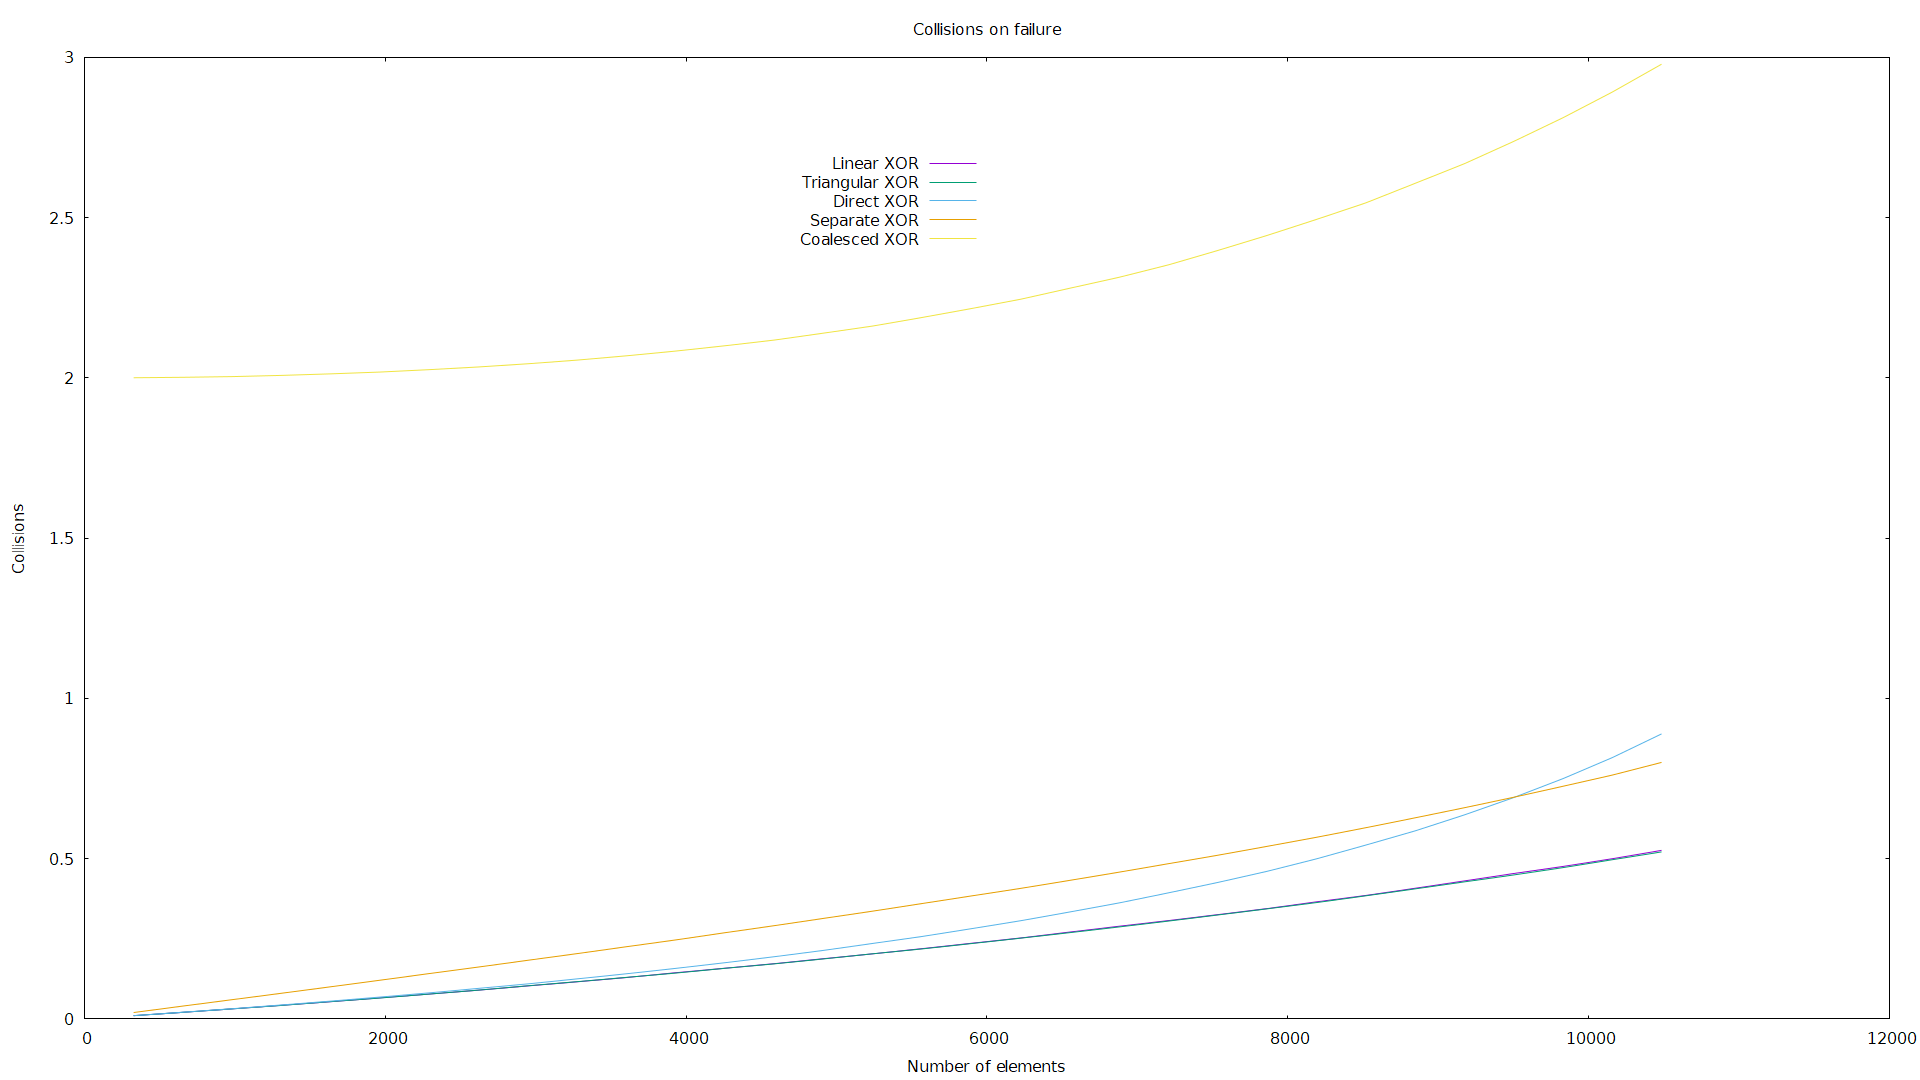
\includegraphics[width=0.7\paperwidth]{Bilder/failure_collisions_part.png}
    \caption{Durchschnittliche Anzahl an Kollisionen bei fehlschlagenden Zugriffen}
\end{figure}
\begin{figure}[h!]
    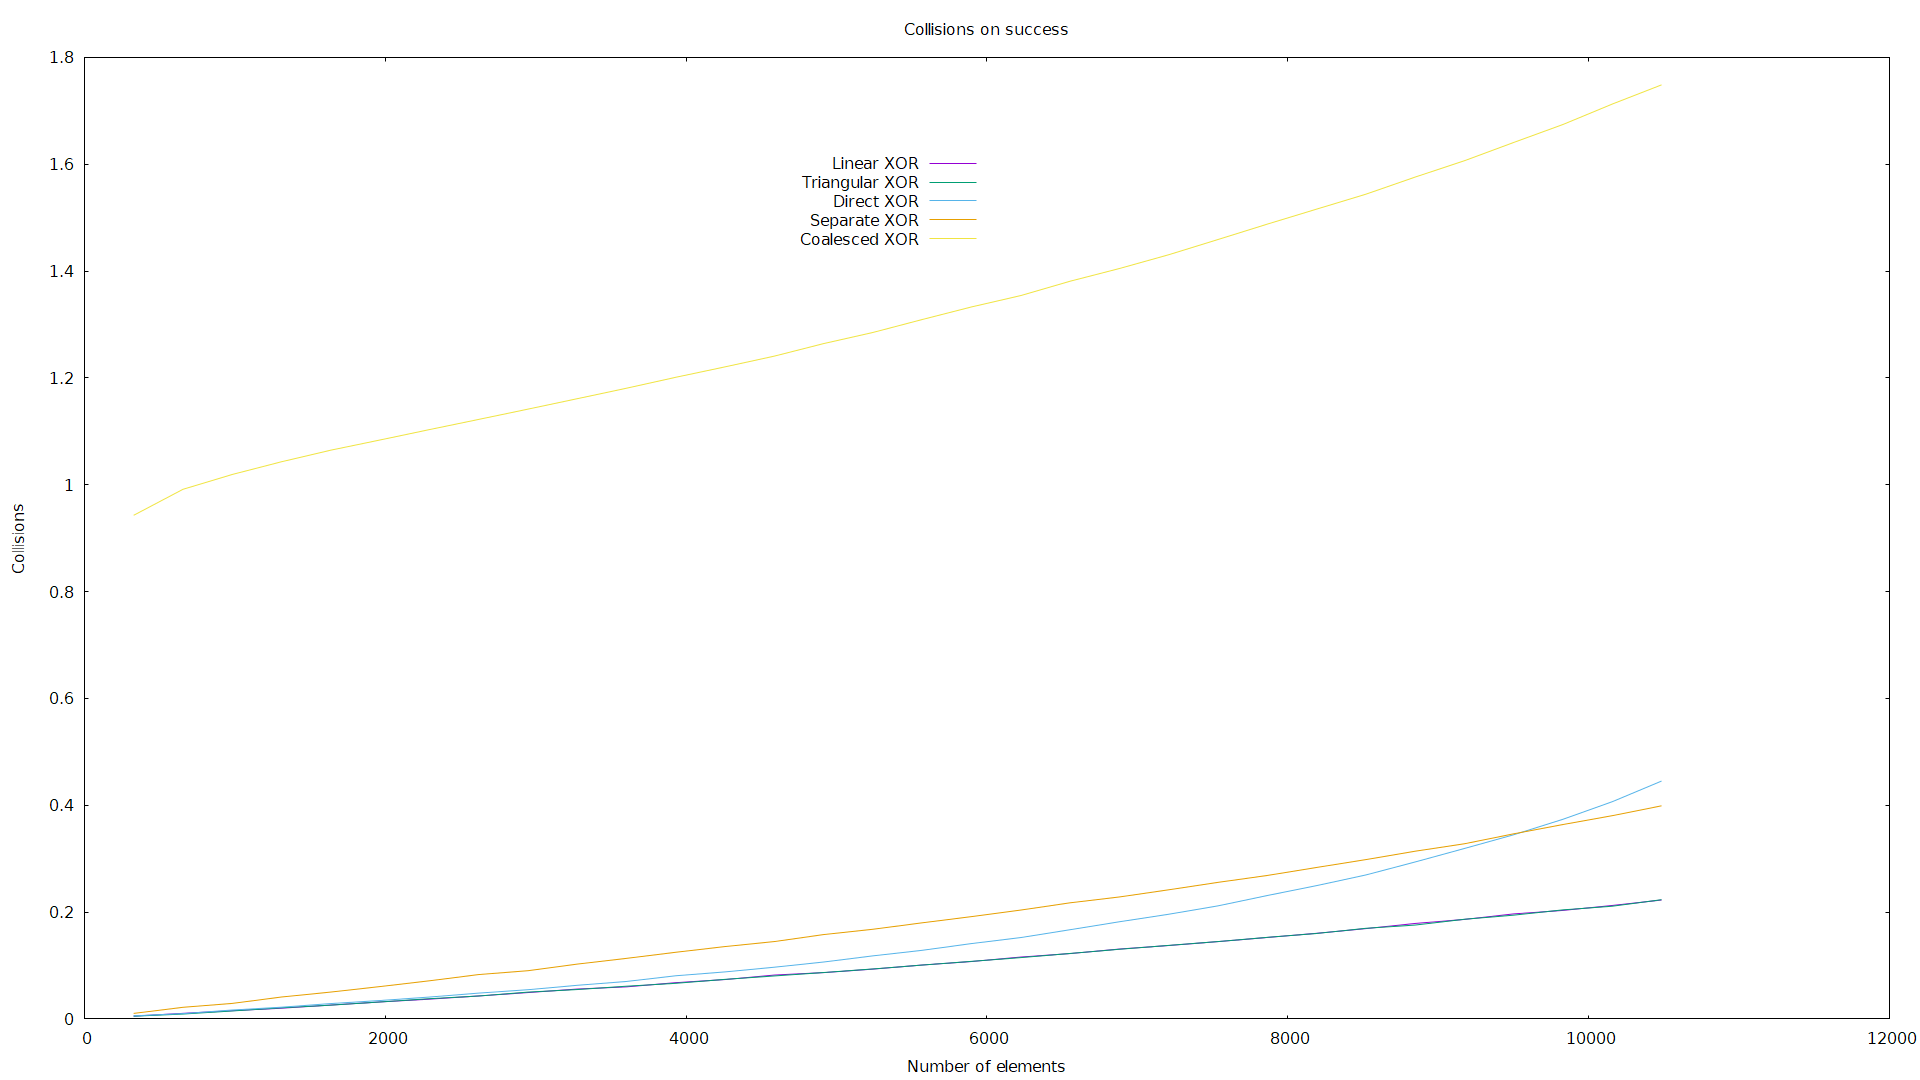
\includegraphics[width=0.7\paperwidth]{Bilder/successful_collisions_part.png}
    \caption{Durchschnittliche Anzahl an Kollisionen bei erfolgreichen Zugriffen}
\end{figure}
\begin{figure}[h!]
    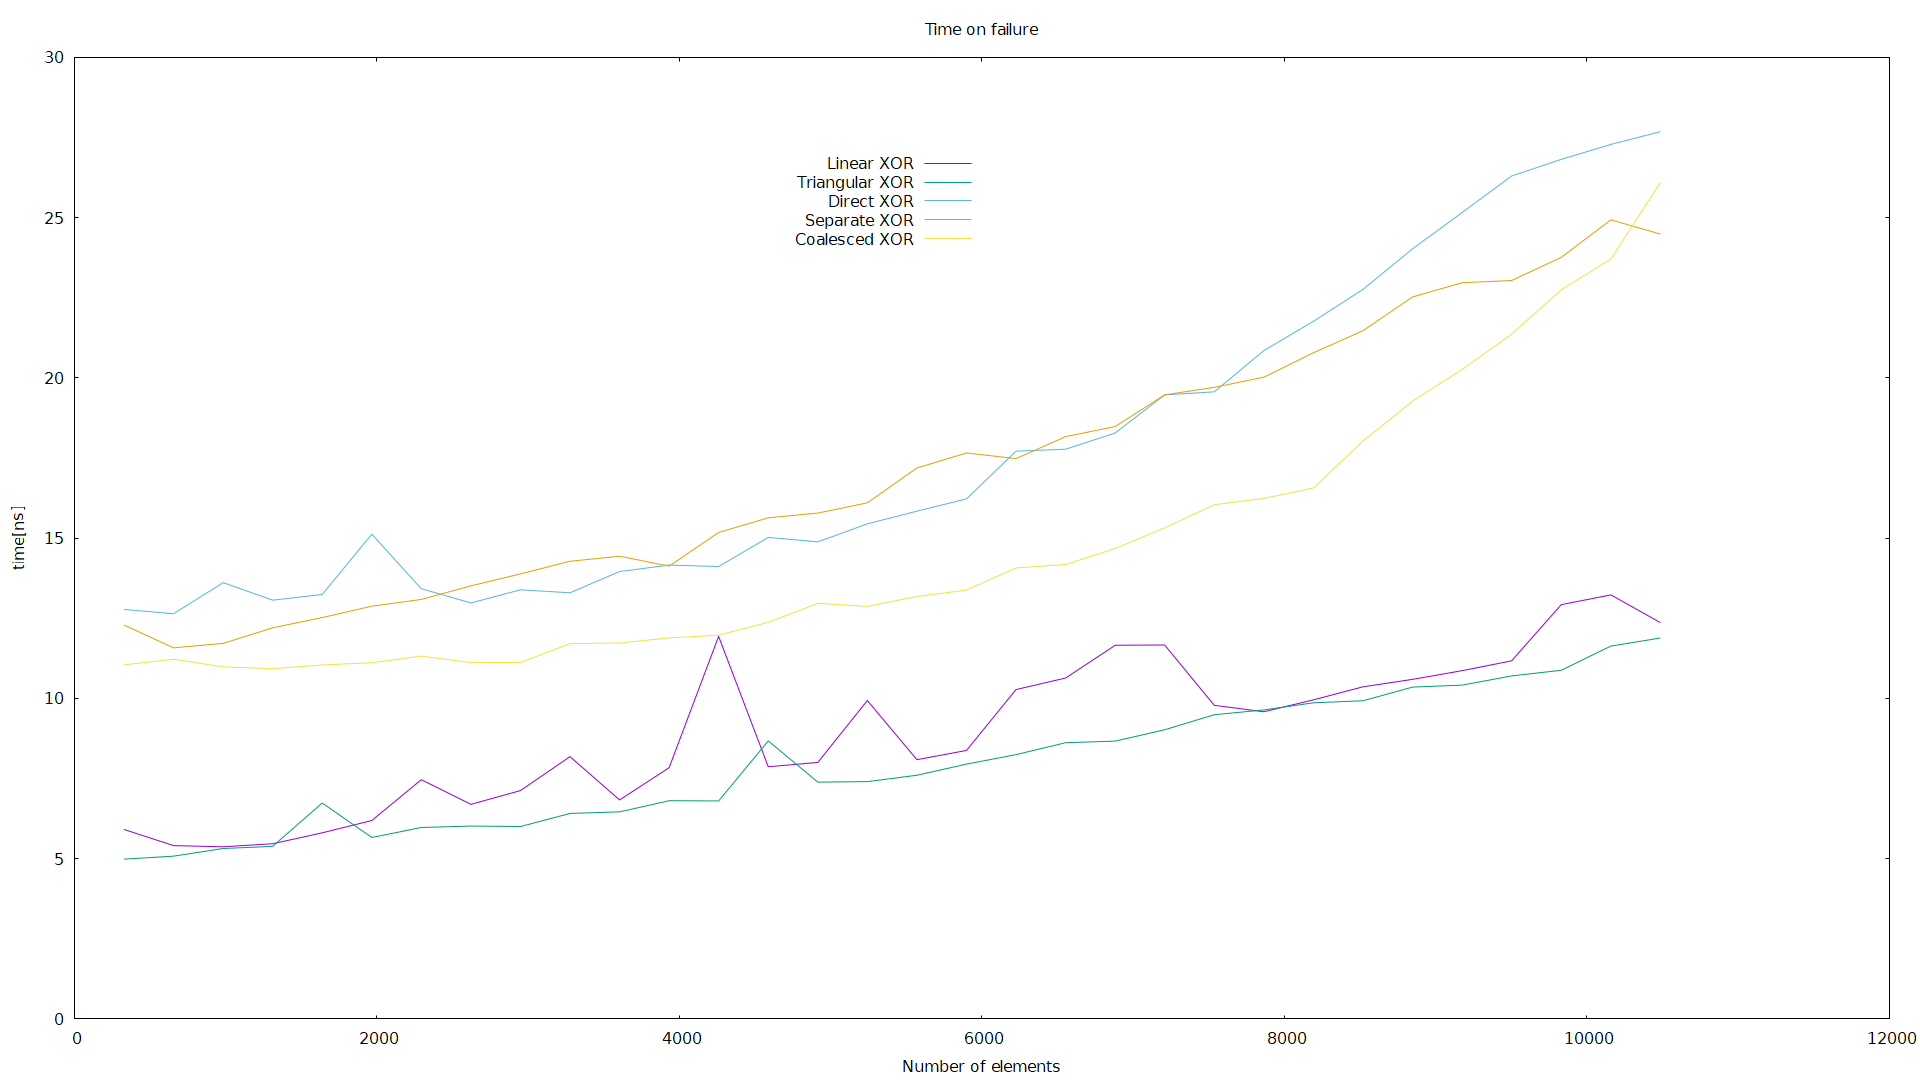
\includegraphics[width=0.7\paperwidth]{Bilder/failure_time_part.png}
    \caption{Durchschnittliche Zugriffszeit bei fehlschlagenden Zugriffen in ns}
\end{figure}
\begin{figure}[h!]
    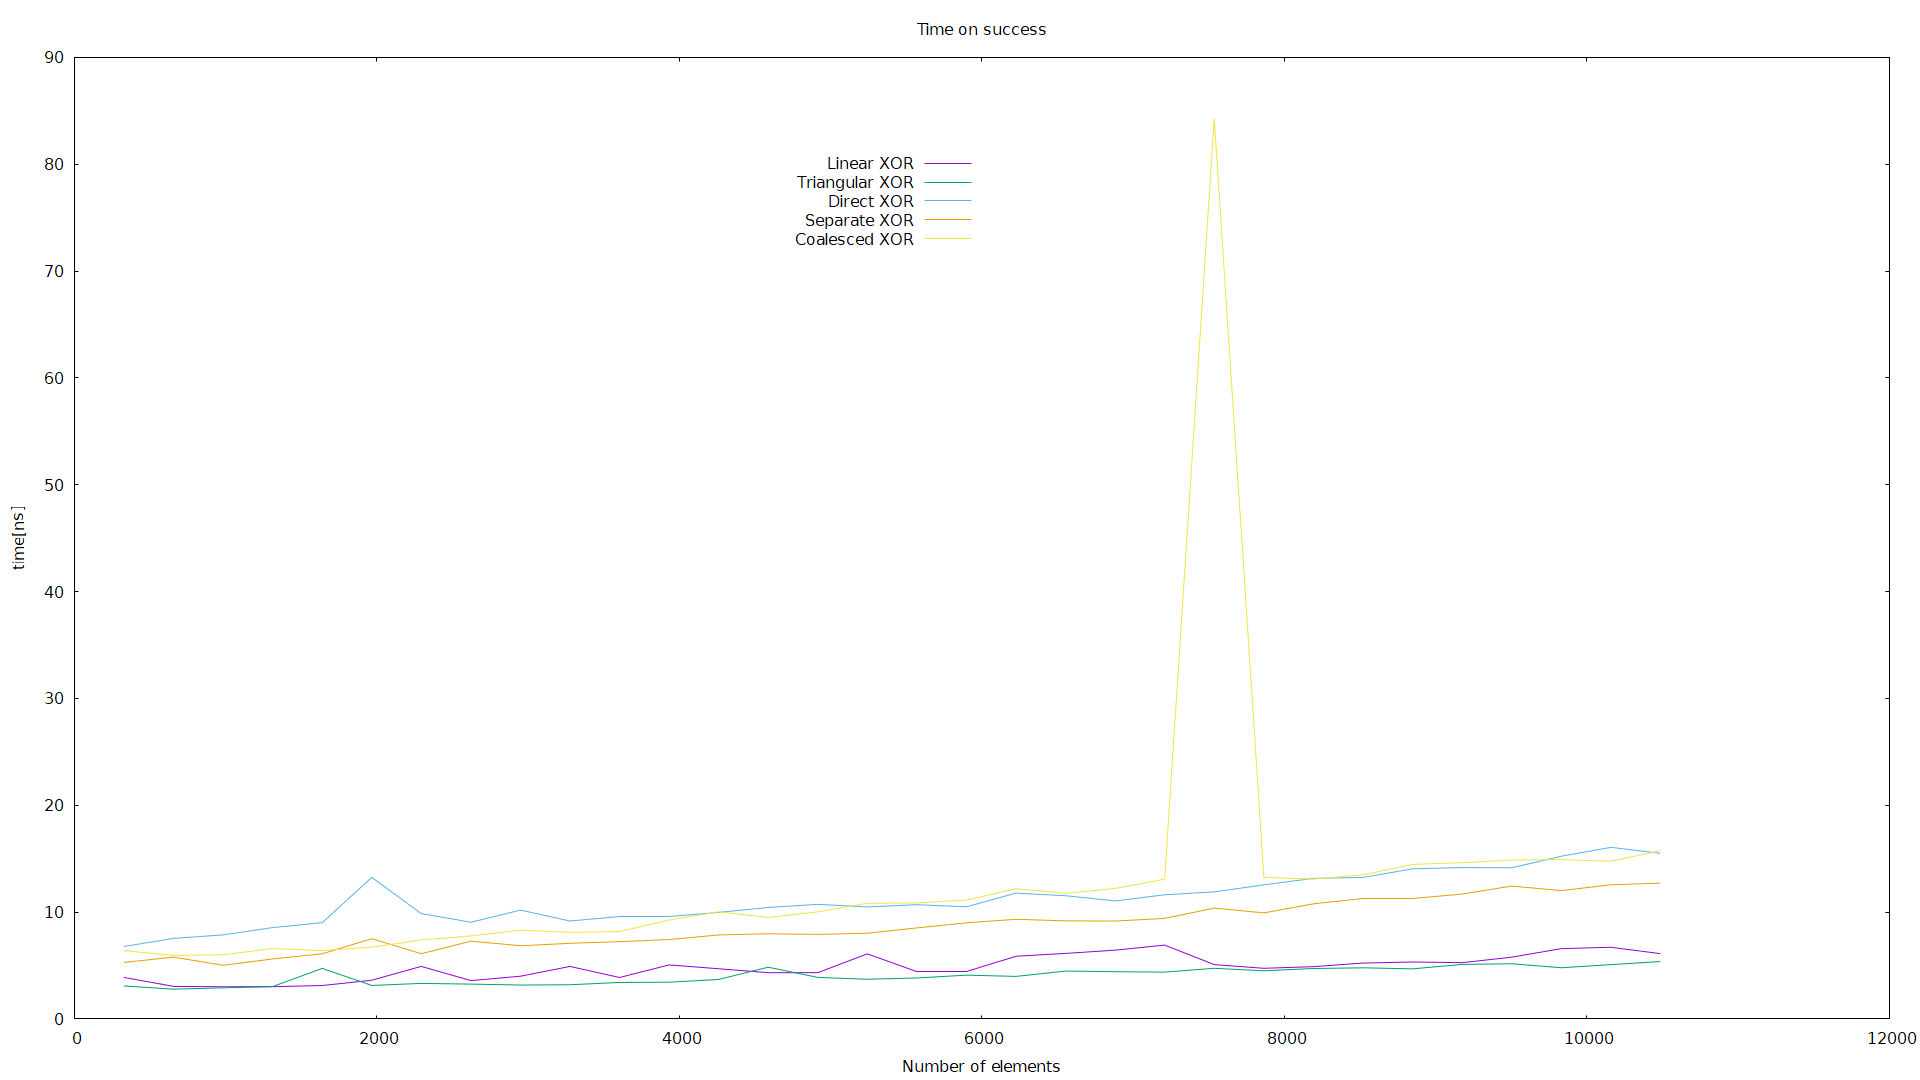
\includegraphics[width=0.7\paperwidth]{Bilder/successful_time_part.png}
    \caption{Durchschnittliche Zugriffszeit bei erfolgreichen Zugriffen in ns}
\end{figure}
\FloatBarrier
\chapter{Interpretation der Ergebnisse}
\section{Interpretation der Egebnisse unter den Bedingungen der Aufgabenstellung}
\section{Interpration der Ergebnisse unter für sinnvoll gehaltenen Bedingungen}
\chapter{Programm- bzw. Quellcode}
\section{Quellcode}
Der komplette Quellcode inklusive Graph-Generierung wurde in Rust geschrieben. Die Ausführung sollte über das Tool \enquote{cargo} durchgeführt werden. Das erhaltene Executable gibt die gemessenen Daten in Tabellenform in stdout aus, erstellt eine csv-Datei mit den Daten und erstellt 4 Graphen. Die Konfiguration der Messung erfolgt über den Quellcode.

Da gefordert wurde, dass der komplette Quellcode im Dokument enthalten ist, hier eine Sektion mit demselben. Alternativ kann das Projekt auch angenehm auf GitHub unter \footnote{https://github.com/imkgerC/uni-theo2-hashset} eingesehen werden. Die Dokumentation und Erklärung des Codes ist über \enquote{Doc Comments} realisiert, kann also im Code durch Kommentare komplett eingebettet gelesen werden. Alternativ kann auch über den Aufruf des Befehls \code{cargo doc} eine HTML-Dokumentation generiert werden.
\section{Vollständiger Quellcode}
\lstinputlisting[label=code:main, caption=main.rs, language=Rust, style=colouredRust]{../src/main.rs}
\lstinputlisting[label=code:mod, caption=mod.rs, language=Rust, style=colouredRust]{../src/hashset/mod.rs}
\lstinputlisting[label=code:hashing, caption=hashing.rs, language=Rust, style=colouredRust]{../src/hashset/hashing.rs}
\lstinputlisting[label=code:probing, caption=probing.rs, language=Rust, style=colouredRust]{../src/hashset/probing.rs}
\lstinputlisting[label=code:chainingtable, caption=chainingtable.rs, language=Rust, style=colouredRust]{../src/hashset/chainingtable.rs}
\lstinputlisting[label=code:openaddressing, caption=openaddressing.rs, language=Rust, style=colouredRust]{../src/hashset/openaddressing.rs}
\lstinputlisting[label=code:coalescedtable, caption=coalescedtable.rs, language=Rust, style=colouredRust]{../src/hashset/coalescedtable.rs}
\lstinputlisting[label=code:logging, caption=logging.rs, language=Rust, style=colouredRust]{../src/logging.rs}


% ---- Literaturverzeichnis
% \cleardoublepage
% \renewcommand*{\chapterpagestyle}{plain}
% \pagestyle{plain}
% \pagenumbering{Roman}                   % Römische Seitenzahlen
% \setcounter{page}{\numexpr\value{savepage}+1}
% \printbibliography[title=Literaturverzeichnis]

% ---- Anhang
% \appendix
%\clearpage
%\pagenumbering{Roman}  % römische Seitenzahlen für Anhang

\newpage
\end{document}
